\documentclass[11pt, a4paper]{article}

\usepackage[utf8]{inputenc}
\usepackage{graphicx}
\graphicspath{ {images/} }
\usepackage{mathtools}
\usepackage{amssymb}
\usepackage{amsmath}
\usepackage[english, ngerman]{babel}
\usepackage{cite}
\usepackage{bibgerm}
\usepackage{fullpage}
\usepackage[top=1.5cm,bottom=1.5cm,left=3.5cm,right=2.5cm,headsep=1.5cm,includeheadfoot]{geometry}
\usepackage{tabularx}
\usepackage{eurosym}
\usepackage{enumitem}
\usepackage{multicol}
\usepackage{tikz}
\usepackage{tkz-euclide}
\usepackage{pgfplots}
\usepackage{pdflscape}
\usepackage{acronym}
\usepackage{blindtext}
\usepackage{ifthen}
\usepackage{setspace}
\usepackage{cancel}
\usepackage{color}
\usepackage{listings}
\usepackage{comment}
\usepackage{xcolor}
\usepackage{colortbl}

\usepackage{fancyhdr}
\pagestyle{fancy}

\fancyhf{} % clear all
\fancyhead[L]{\leftmark}
\fancyfoot[C]{-- \thepage{} --}
%\setlength{\headheight}{15pt}
\renewcommand{\headrulewidth}{0.5pt}
\renewcommand{\footrulewidth}{0pt}
\setlength{\skip\footins}{0.7cm}

\usetikzlibrary{graphs}
\usetikzlibrary{positioning}

\onehalfspacing
\setlength\parindent{0pt}

%\everymath{\displaystyle}

\allowdisplaybreaks

\definecolor{AI-BLUE}{rgb}{0,0.57,0.87}

% Eigene Befehle
\newcommand\q[1]{\glqq{}#1\grqq{}}
\renewcommand\equiv{\Leftrightarrow}
\newcommand\vertequal[2]{\underset{\underset{#2}{\parallel}}{#1}}
\newcommand\cif{\text{if }}
\newcommand\abs[1]{\left|#1\right|}
\newcommand\norm[1]{\abs{\abs{#1}}}
\newcommand\diff[1]{\text{ d#1}}
\newcommand\av[1]{\left\langle#1\right\rangle}
\newcommand\ev[1]{\mathbb{E}\left(#1\right)}
\newcommand\br[1]{\left(#1\right)}
\newcommand\ubr[2]{\underbrace{#1}_{#2}}
\newcommand\quer[1]{\overline{#1}}
\newcommand\setequal{\overset{!}{=}}
\newcommand\dint{\displaystyle \int}
\newcommand\dsum{\displaystyle \sum}
\newcommand\dprod{\displaystyle \prod}
\newcommand\closedInt[2]{\left[#1,#2\right]}
\newcommand{\checkbox}{\Large \Square \normalsize \hspace{0.4cm}}

\newcommand\myref[1]{\ref{#1} (S. \pageref{#1})}
\newcommand\myrefcomma[1]{\ref{#1}, S. \pageref{#1}}

\newcommand\nsm{Nagel-Schreckenberg-Modell }

\begin{document}

\thispagestyle{empty}

\pagenumbering{Roman}

\setlength{\hoffset}{-0.5cm} % center title page

\begin{titlepage}
    \begin{center}
    \vphantom{0cm}
    \LARGE \textbf{Dokumentation}\\
    \vspace{3cm}
    \normalsize
    Dokumentation für Simulationstechnik \\
    im Master-Studiengang \textcolor{AI-BLUE}{[Angewandte Informatik]}\\
    an der Ruhr-Universität Bochum\\
    im Wintersemester 2014/15\\
    \vspace{4cm}
    \huge \textbf{Verkehrssimulation mit Zellularautomaten in C++} \\
    \vspace{4cm}
    \normalsize
    \textbf{Projektteilnehmer:}\\
    B. Sc. Christian Andreas Mielers (108 011 204 956)\\
    B. Sc. Phil Yannick Schrör (108 011 214 024)\\
    \vspace{2cm}
    \textbf{Projektbetreuer:}\\
    M. Sc. Markus Scheffer
    \end{center}
\end{titlepage}

\newpage
\tableofcontents

\newpage
\pagenumbering{arabic}

\section{Einleitung}
\label{sec:einleitung}

\newpage
\section{Annahmen}
\label{sec:ansatz}

Im Groben basiert unser Modell auf den Annahmen, die Kai Nagel und Michael Schreckenberg \cite{nagel-schreckenberg} für ihr Verkehrsmodell getroffen haben. Um das Modell jedoch an die Verhältnisse auf deutschen Straßen anzupassen, wurden einige Änderungen vorgenommen.
Im Folgenden werden die unserem Modell zugrunde liegenden Annahmen aufgeführt:

\begin{itemize}
\item Es gilt weiterhin, dass eine Zelle 7,5 Meter lang ist und jede Zelle nur ein einziges Fahrzeug zur gleichen Zeit aufnehmen kann.
\item Im klassichen \nsm gibt es die Geschwindigkeitsstufen 0 bis 5. Diese entsprechen Geschwindigkeiten von 0 km/h bis 135 km/h in 27 km/h Abschnitten. Da uns 135 km/h als Höchstgeschwindigkeit auf einer deutschen Autobahn als zu wenig erschienen, haben wir die Höchstgeschwindigkeit auf 7 erhöht, so dass Fahrzeuge nun eine Maximalgeschwindigkeit von 189 km/h erreichen können.
\item Während im \nsm alle Fahrzeuge üblicherweise die gleiche Maximalgeschwindigkeit erreichen können, werden in unserem Modell die Maximalgeschwindigkeiten der Fahrzeuge aus einer Normalverteilung gezogen, deren Mittelwert und Standardabweichung vom Nutzer des Programms frei gewählt werden können. Falls vom Nutzer keine Varianz bei den Maximalgeschwindigkeiten gewünscht ist, kann er die Standardabweichung sehr klein wählen, so dass es sehr unwahrscheinlich wird, eine Maximalgeschwindigkeit ungleich dem Mittelwert zu erhalten. Es ist zu beachten, dass es nicht möglich ist, Fahrzeugen Maximalgeschwindigkeiten zuzuweisen, die 3 unter- oder 7 überschreiten. Dies ist dadurch begründet, dass in Deutschland nur solche Fahrzeuge eine Autobahn befahren dürfen, welche eine Höchstgeschwindigkeit von mindestens 60 km/h erreichen können. Ein Fahrzeug mit der Geschwingkeitsstufe 2 als Höchstgeschwindigkeit (= 54 km/h) würde diesen Grenzwert um 6 km/h unterschreiten.
\item Um unterschiedliche Fahrertypen abbilden zu können, wird der Trödelfaktor eines jeden Fahrzeugs ebenfalls randomisiert bestimmt. Zu diesem Zweck wird jedoch keine Normalverteilung verwendet, sondern eine Gleichverteilung, deren Minimalwert und Maximalwert ebenfalls frei vom Nutzer festgelegt werden kann. Ist auch hier keine Varianz erwünscht, kann der Minimalwert gleich dem Maximalwert gewählt werden. Als Grenzen für den Trödelfaktor gelten nur die natürlichen Schranken 0 und 1. Zu hohe Trödelfaktoren sollten jedoch nicht verwendet werden, da das System sonst schnell zum Stillstand kommt.
\end{itemize}

\newpage
\section{Umsetzung}
\label{sec:umsetzung}

\subsection{Autobahn}
\label{subsec:umsetzung-autobahn}

Wir haben unser Modell für die Simulation von Autobahnen strukturell für beliebig viele Spuren ausgelegt. Die in der Aufgabenstellung unterschiedenen Simulationsexperimente einer einspurigen bzw. einer zweispurigen Autobahn können also mit der gleichen Simulationssoftware durchgeführt werden. Somit wird im Folgenden die Umsetzung dieses Modells nur im Allgemeinen beschrieben, nicht jedoch für die genannten Spezialfälle.

Als Repräsentation für die Autobahn dient eine $l \times s$ Matrix, wobei $l$ die Anzahl Spuren und $s$ die Anzahl der Straßensegmente angibt. Für die Simulation einer 2,25km langen Autobahn mit drei Spuren wird also eine $3 \times 300$ Matrix erzeugt. Im Wesentlichen dient diese Matrix dazu, Fahrzeuge und ihre Position auf der Autobahn zu speichern.


\subsection{Kreisverkehr (und beliebige Straßenverläufe)}
\label{subsec:umsetzung-kreisverkehr}

Ein dritter Teil der Aufgabenstellung bestand darin, den Verkehrsfluss eines Kreisverkehrs zu simulieren. Dies ist ein ungleich schwierigeres Problem, da es hier an einigen Stellen Verzweigungen und Zusammenführungen geben kann, bei denen Kollisionsfreiheit gewährleistet werden muss. Zwar kann man den Spurwechsel auf der mehrspurigen Straße auch als Verzweigung/Zusammenführung betrachten, allerdings weist dieser Gleichmäßigkeit über alle Zellen hinweg auf, d.h. die Regeln können einmalig, relativ zur Zellposition und den Geschwindigkeiten der Fahrzeuge festgelegt werden. Im Kreisverkehr hingegen verhalten sich einige Zellen deutlich anders als andere, beispielsweise hinsichtlich zulässiger Geschwindigkeit oder Anzahl der Richtungen, in die man sich bewegen kann. In diesem Zusammenhang müssen auch Vorfahrtsregeln beachtet werden. Darüber hinaus haben Ereignisse in einer Zelle (z.B. die Entscheidung, eine Ausfahrt zu nehmen) Auswirkungen auf die Handlungsmöglichkeiten der Autos in den umliegenden Zellen. Diese Anforderungen machen einen erheblich dynamischeres Vorgehen bei der Berechnung der Bewegungen der Fahrzeuge erforderlich. Eine Lösung muss also folgende Anforderungen erfüllen:

\begin{enumerate}
	\item Kollisionsfreiheit
	\item Vorfahrtsregeln
	\item Geschwindigkeitsbegrenzungen
\end{enumerate}

Grundsätzlich wäre eine vergleichsweise simple Lösung möglich, die die Anforderungen dieses spezifischen Szenarios erfüllt. Hierbei würde man die kritischen Stellen, wie die Zu- und Abfahrtszellen zum/vom Kreisverkehr, gesondert behandeln und dafür eine andere Logik implementieren. Es ist offensichtlich, dass eine solche Lösung hochgradig abhängig vom der Problemstellung ist und man daher für jedes Szenario manuelle Anpassungen vornehmen muss. Dies ist nicht zufriedenstellend, weswegen wir uns ein Verfahren zum Ziel gesetzt haben, dass von Spezifika des Scenarios (wie der konkreten Position der Abzweigungen) unabhängig ist.

Strukturell behalten wir das Layout eines Grids bei, in dem die Zellen der Simulation mit x- und y-Koordinaten gespeichert werden. Dies dient allerdings nur der Vereinfachung der Visualisierung. Konzeptionell besteht unsere Straßenkarte aus losen Zellen, die Verweise auf ihre Vorgänger- und Nachfolgerzellen beinhalten. Somit entspricht das Layout unserer Lösung einem gerichteten, nicht notwendigerweise kreisfreien Graphen.

Zunächst betrachten wir die Anforderung der Kollisionsfreiheit. Es soll, analog zum Nagel-Schreckenberg Modell \cite{nagel-schreckenberg} erreicht werden, dass in keinem Simulationsschritt eine Zelle von mehr als einem Auto befahren wird. Ein einfacher Weg dies zu erreichen besteht darin, alle Fahrzeuge sequenziell durchzugehen und für jedes die Zellen, die es abfahren möchte zu markieren. Hier geht man nur soweit, wie das Auto mit seiner aktuellen Geschwindigkeit fahren kann. Dabei wird das Markieren gestoppt, sobald eine Zelle erreicht wird, die bereits von einem anderen Auto markiert wurde. Nachdem alle Fahrzeuge ihren Weg markiert haben, wird für jedes die Anzahl der Markierungen gezählt und seine Geschwindigkeit auf diese Zahl gedeckelt.

Bei diesem Ansatz ergibt sich allerdings das Problem, dass Vorfahrtsregeln missachtet werden. Wird zuerst ein Fahrzeug bewegt, dass dann von einer Nebenstraße aus in eine Hauptstraße eingibt und dort Zellen markiert, blockiert es dort möglicherweise ein Vorfahrt habendes Fahrzeug. Es gibt keine Möglichkeit präemtiv zu bestimmen, welches Fahrzeug Vorfahrt haben wird. Das kann man unter Anderem daran sehen, dass die Vorfahrts-Relation nicht transitiv ist (vgl. Abb. \ref{fig:rightOfWayNotTransitive}), weswegen keine Ordungsrelation auf den Fahrzeugen etabliert werden kann. Daher muss es eine Möglichkeit geben, Markierungen zu überschreiben. Der Ansatz wird also so erweitert, dass ein Fahrzeug nur dann mit dem Markieren aufhört, wenn es an einer Zusammenführung auf eine Markierung trifft, ohne an der Zusammenführung Vorfahrt gehabt zu haben. Hat es Vorfahrt, überschreibt es die Markierungen einfach. Die Vorfahrt wird über die Reihenfolge der Vorgängerverweise einer Zelle bestimmt, ist also eine lokale Eigenschaft. Externe Informationen sind nicht erforderlich. Da die Geschwindigkeit der Fahrzeuge erst berechnet wird nachdem alle Autos abgearbeitet wurden, lassen sich mit dieser Methode Vorfahrtsregeln berücksichtigen. Die Kollisionsfreiheit bleibt dabei erhalten.
\begin{figure}[h!]
	\centering
	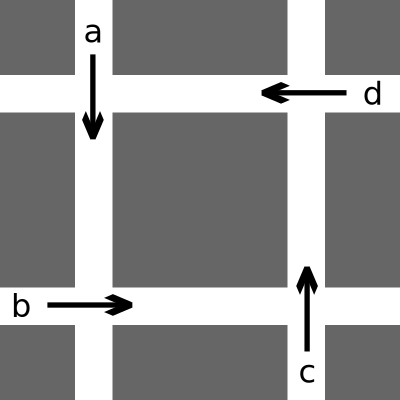
\includegraphics[width=6cm]{img/rightOfWay}
	\caption{Vorfahrt ist nicht transitiv: d hat Vorfahrt vor c hat Vorfahrt vor b hat Vorfahrt vor a hat Vorfahrt vor d}
	\label{fig:rightOfWayNotTransitive}
\end{figure}

Ein Problem beim Überschreiben ist jedoch, dass 'Stummel' vorheriger Markierungen übrig bleiben können. Daher müssen, wenn eine Markierung eines Fahrzeugs entfernt wird, alle Markierungen des Fahrzeugs entfernt werden. Später sind dann die Markierungen des Fahrzeuges neu zu bestimmen.
\begin{figure}[h!]
	\centering
	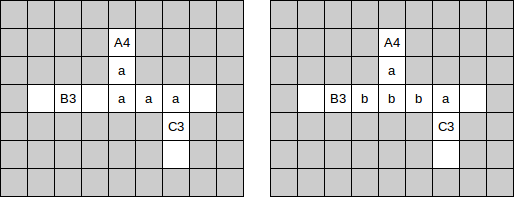
\includegraphics[width=8cm]{img/stubs}
	\caption{Möglichkeit von Stummeln: Links: A markiert zunächst 4 Felder. Dann rechts: B hat vorfahrt, markiert dabei 3 Felder und überschreibt Markierungen von A. Übberreste der Markierungen von A behindern nun C, der eigentlich fahren könnte}
	\label{fig:rightOfWayNotTransitive}
\end{figure}

Zuletzt muss noch die Anforderung des Einhaltens von Geschwindigkeitsbegrenzungen erfüllt werden. Dazu wird jede Zelle mit einer Maximalgeschwindigkeit versehen. Betritt ein Fahrzeug eine Zelle, wird die maximale Anzahl an Zellen, die es darüber hinaus noch markieren kann auf die Maximalgeschwindigkeit der Zelle gedeckelt. Somit ist gewährleistet, dass kein Fahrzeug an keiner Zelle die zulässige Geschwindigkeit überschreitet.

Diese Überlegungen führen zu folgendem Markierungsalgorithmus:
\lstinputlisting[numbers=right]{src/streetMapMarkAlgorithm}
wobei r die verbleibenden Schritte des Autos runterzählt. Ob ein Fahrzeug an einer Zusammenführung Vorfahrt hat, ergibt sich wie oben beschrieben aus der Reihenfolge der Vorgängerverweise. Um die Implementierung zu vereinfachen beschränken wir uns auf Zusammenführungen mit zwei Vorgängern.

Nachdem die Markierungen entsprechend gesetzt wurden müssen im Anschluss daran aus ihnen die tatsächlichen Fahrdistanzen für die einzelnen Fahrzeuge berechnet werden. Dazu kann man in jedem Fahrzeug starten und seine Wunschstrecke solange ablaufen, wie man dabei nur vom Fahrzeug markierte Zellen betritt. Hierbei zählt man eine Variable hoch, die am Ende die Geschwindigkeit des Fahrzeuges angibt. Dies geschieht folgendermaßen:
\lstinputlisting[numbers=right]{src/streetMapDistAlgorithm}

Damit haben wir einen Algorithmus erreicht, der beliebige Verkehrsnetze kollisionsfrei unter Berücksichtigung von Vorfahrtsregeln und Geschwindigkeitsbegrenzungen simulieren kann. Im Kontrast zur mehrspurigen Simulation oben kann dieses Verfahren zwar ebenfalls mit mehreren Spuren umgehen, das Rechtsfahrgebot und das Rechtsüberholverbot müssten aber separat implementiert werden. Bis auf das modifizierte Verfahren zur Bestimmung der maximalen Fahrdistanz können die Regeln des Nagel-Schreckenberg Modells \cite{nagel-schreckenberg} übernommen werden. Es werden also zunächst alle Fahrzeuge beschleunigt, dann die Distanzen wie oben beschrieben geprüft, anschließend getrödelt und am Ende die Fahrzeuge bewegt.

Eine schöne Eigenschaft dieser Herangehensweise ist, dass wir ohne zusätzlichen Aufwand Quellen und Senken von Fahrzeugen erzeugen können. Als Quelle wird schlicht jede Zelle definiert, die zwar Nachfolger, aber keine Vorgänger hat. Analog ist jede Zelle eine Senke, die Vorgänger, aber keine Nachfolger hat. Jeder Zelle kann darüber hinaus eine Autoerzeugungswahrscheinlichkeit zugeordnet werden, mit der in der Zelle pro Simulationsschritt ein neues Auto entsteht, sofern sie leer ist. Ein Auto, was eine Senke überfährt, wird hingegen entfernt.

Nun bleibt noch die Frage zu klären, wie an einer Verzweigung die Entscheidung zu treffen ist, in welche Richtung ein Fahrzeug fahren soll (vgl. Zeile 7). Konzeptionell wäre es möglich, jedem neu hinzugefügten Fahrzeug ein Ziel zuzuweisen und einen (randomisierten) Pfadfindungsalgorithmus zu nutzen, um die Entscheidungen an Verzweigungen zu treffen. Da Fahrzeuge in der Regel ein festes Ziel haben, wäre dies der realistischste Ansatz. Zur Vereinfachung der Implementierung entscheiden wir uns allerdings dafür, die Entscheidung an jeder Verzweigung zufällig zu treffen, wobei für jede Nachfolgerzelle individuelle Wahrscheinlichkeiten festgelegt werden können. Da wir nur sehr einfache Straßennetze mit wenigen Verzweigungen (die insbesondere nicht verschachtelt sind) betrachten, erachten wir das als eine ausreichend gute Annäherung. Für komplexere Szenarien werden allerdings komplexere Entscheidungssysteme notwendig.

%TODO: Problem: wenn wir markierungen überschreiben, können 'Stummel' überbleiben, die andere Fahrzeuge blockieren. Illustrieren

\newpage
\section{Ergebnisse}
\label{sec:ergebnisse}
\subsection{Einspurige Straße}
\subsection{Mehrspurige Straße}
\subsection{Kreisverkehr}
Bei der Simulation des Verkehrsflusses an einem Kresverkehr gibt es Verzweigungen und Zusammenführungen, wobei Vorfahrtsregeln und Geschwindigkeitsbegrenzungen zu beachten sind. Daher wird das in Abschnitt \ref{subsec:umsetzung-kreisverkehr} entwickelte Verfahren benutzt. Simuliert wird ein Kreisverkehr mit \texttt{8 Zellen Breite} und \texttt{6 Zellen Höhe}, es handelt sich also näherungsweise um ein Rechteck mit \texttt{60m} Breite und \texttt{45m} Höhe, da wir weiterhin von einer Zellenlänge von $7.5m$ ausgehen. Zum Kreisverkehr führen \texttt{3 Zubringerstraßen bzw. Ausfahrten} die von links, rechts und unten kommen, dementsprechend gibt es \texttt{3 Quellen} und \texttt{3 Senken}. An der Oberseite befinden sich keine Abzweigungen, der Kreisverkehr weist also eine Asymmetrie auf. Die Länge der Zu- und Abfahrten kann variiert werden. Wir entschließen uns dazu, sie auf \texttt{20 Zellen} zu setzen. Zusätzlich gilt die Forderung, dass Fahrzeuge nur mit einer Geschwindigkeit von \texttt{einer Zelle pro Sekunde} in den Kreisverkehr einfahren dürfen, was einer Realgeschwindigkeit von $27km/h$ entspricht. Aufgrund der Proportionen des Kreisverkehrs erscheint es uns auch angemessen, die Geschwindigkeit innerhalb des Kreisverkehrs auf diesen Wert zu beschränken. Da wir von einer Landstraße ausgehen setzen wir das Limit für die Zu- und Abfahrten auf \texttt{4 Zellen/Sekunde}, was $108km/h$ entspricht. Damit ergibt sich die in Abbildung  zu sehende schematische Darstellung der Straßenkarte.

\begin{figure}[h!]
	\centering
	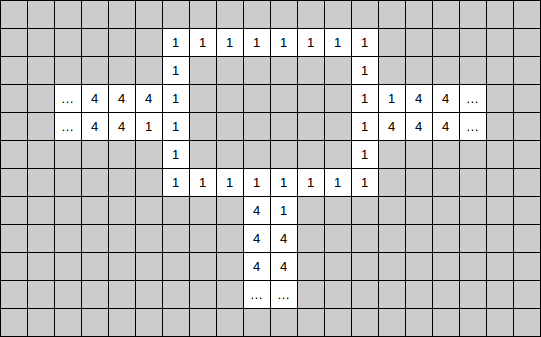
\includegraphics[width=8cm]{img/roundaboutSmall}
	\caption{Möglichkeit von Stummeln: Kreisverkehr mit eingetragenen Höchstgeschwindigkeiten}
	\label{fig:roundaboutSmall}
\end{figure}

Schließlich müssen wir noch die Wahrscheinlichkeit, den Kreisverkehr an jeder der Verzweigungen zu verlassen definieren. Diese wird auf \texttt{1/3} gesetzt, was dazu führt dass die Wahrscheinlichkeit, die erste oder die zweite Ausfahrt zu nehmen näherungsweise gleich ist, bei der dritten Ausfahrt (wo das Fahrzeug hergekommen ist), aber signifikant geringer.

\subsection{Autobahnkreuz}

\newpage
\section{Fazit}
\label{sec:fazit}

\blindtext asdf \cite{mehrspurig}\\
In Kapitel \myref{sec:einleitung} steht Shit. In Foobar (\myrefcomma{sec:ansatz}) bla

\newpage
\addcontentsline{toc}{section}{Literatur}
\bibliography{ref}{}
\bibliographystyle{alpha}

\end{document}